The oscillations produced without an added damping factor, i.e. the magnet are displayed in \label{fig:undamped oscillations}. The assumption was made that the string to which the springs were attached did not slip from the pulley. Figure 2 shows underdamped oscillations, which can be seen by a decrease in amplitudes.

\begin{figure}[h!]
  \centering
  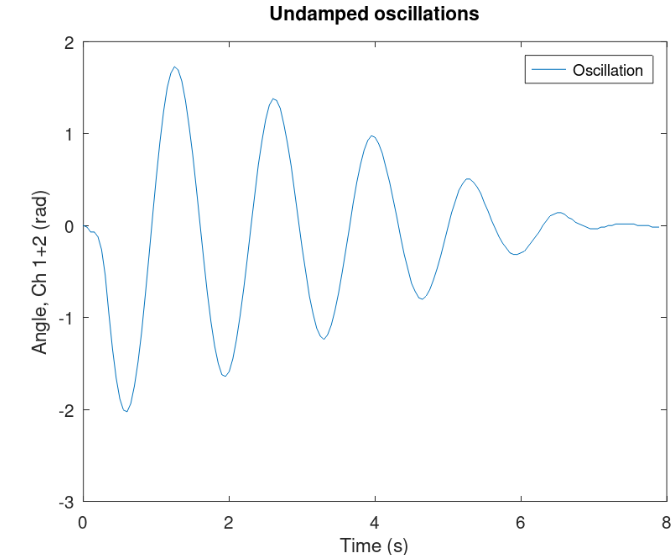
\includegraphics[width=1\textwidth]{oscillations/images/Undamped Oscillations}
  \caption{Oscillations without damping}
  \label{fig:undamped oscillations}
\end{figure}

From the measurements the coordinates of the maxima were determined and from this the natural frequency was determined to be 4.8 +- 0.1 rad/s, which was constant throughout the measurements.

A damping term was added by placing the magnet back in its original position, the oscillations are displayed in Figure 3. The coordinates of nine of the maxima were determined and were plotted in \label{log of damping factor}. 

\begin{figure}[h!]
  \centering
  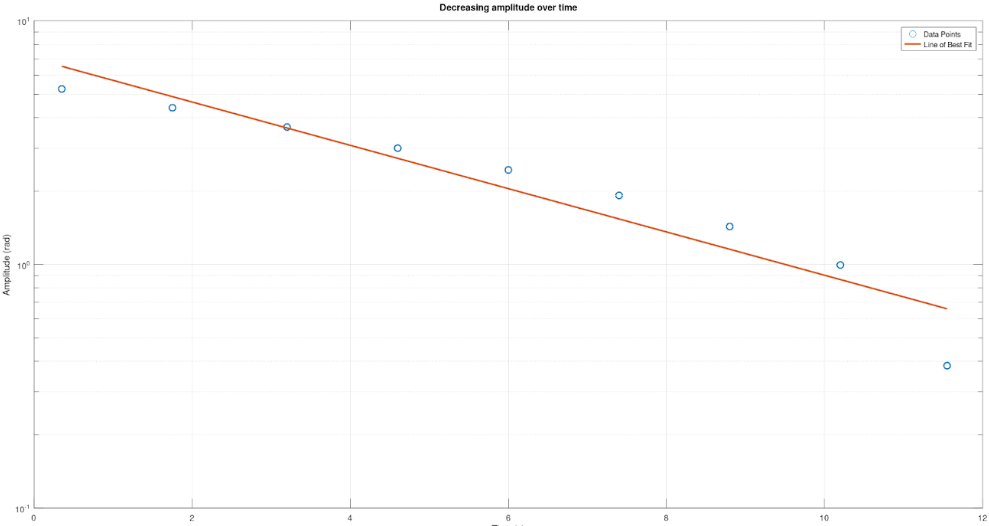
\includegraphics[width=1\textwidth]{oscillations/images/Log of damping factor}
  \caption{Semi-logaritmic plot of the amplitude over time}
  \label{log of damping factor}
\end{figure}

The displacement amplitude $x(t)$ decreases with:
\begin{equation}
  x(t) = e^{-\gamma t} \cos(\omega t + \phi) 
\end{equation}
The slope of the line of best fit $l$ is equal to the $-\gamma$ term in Equation .
\begin{equation}
  |l| = \gamma 
\end{equation}
By this a damping factor of $1.3 ± 0.2$ rad/s was determined.



\begin{figure}[H]
  \centering
  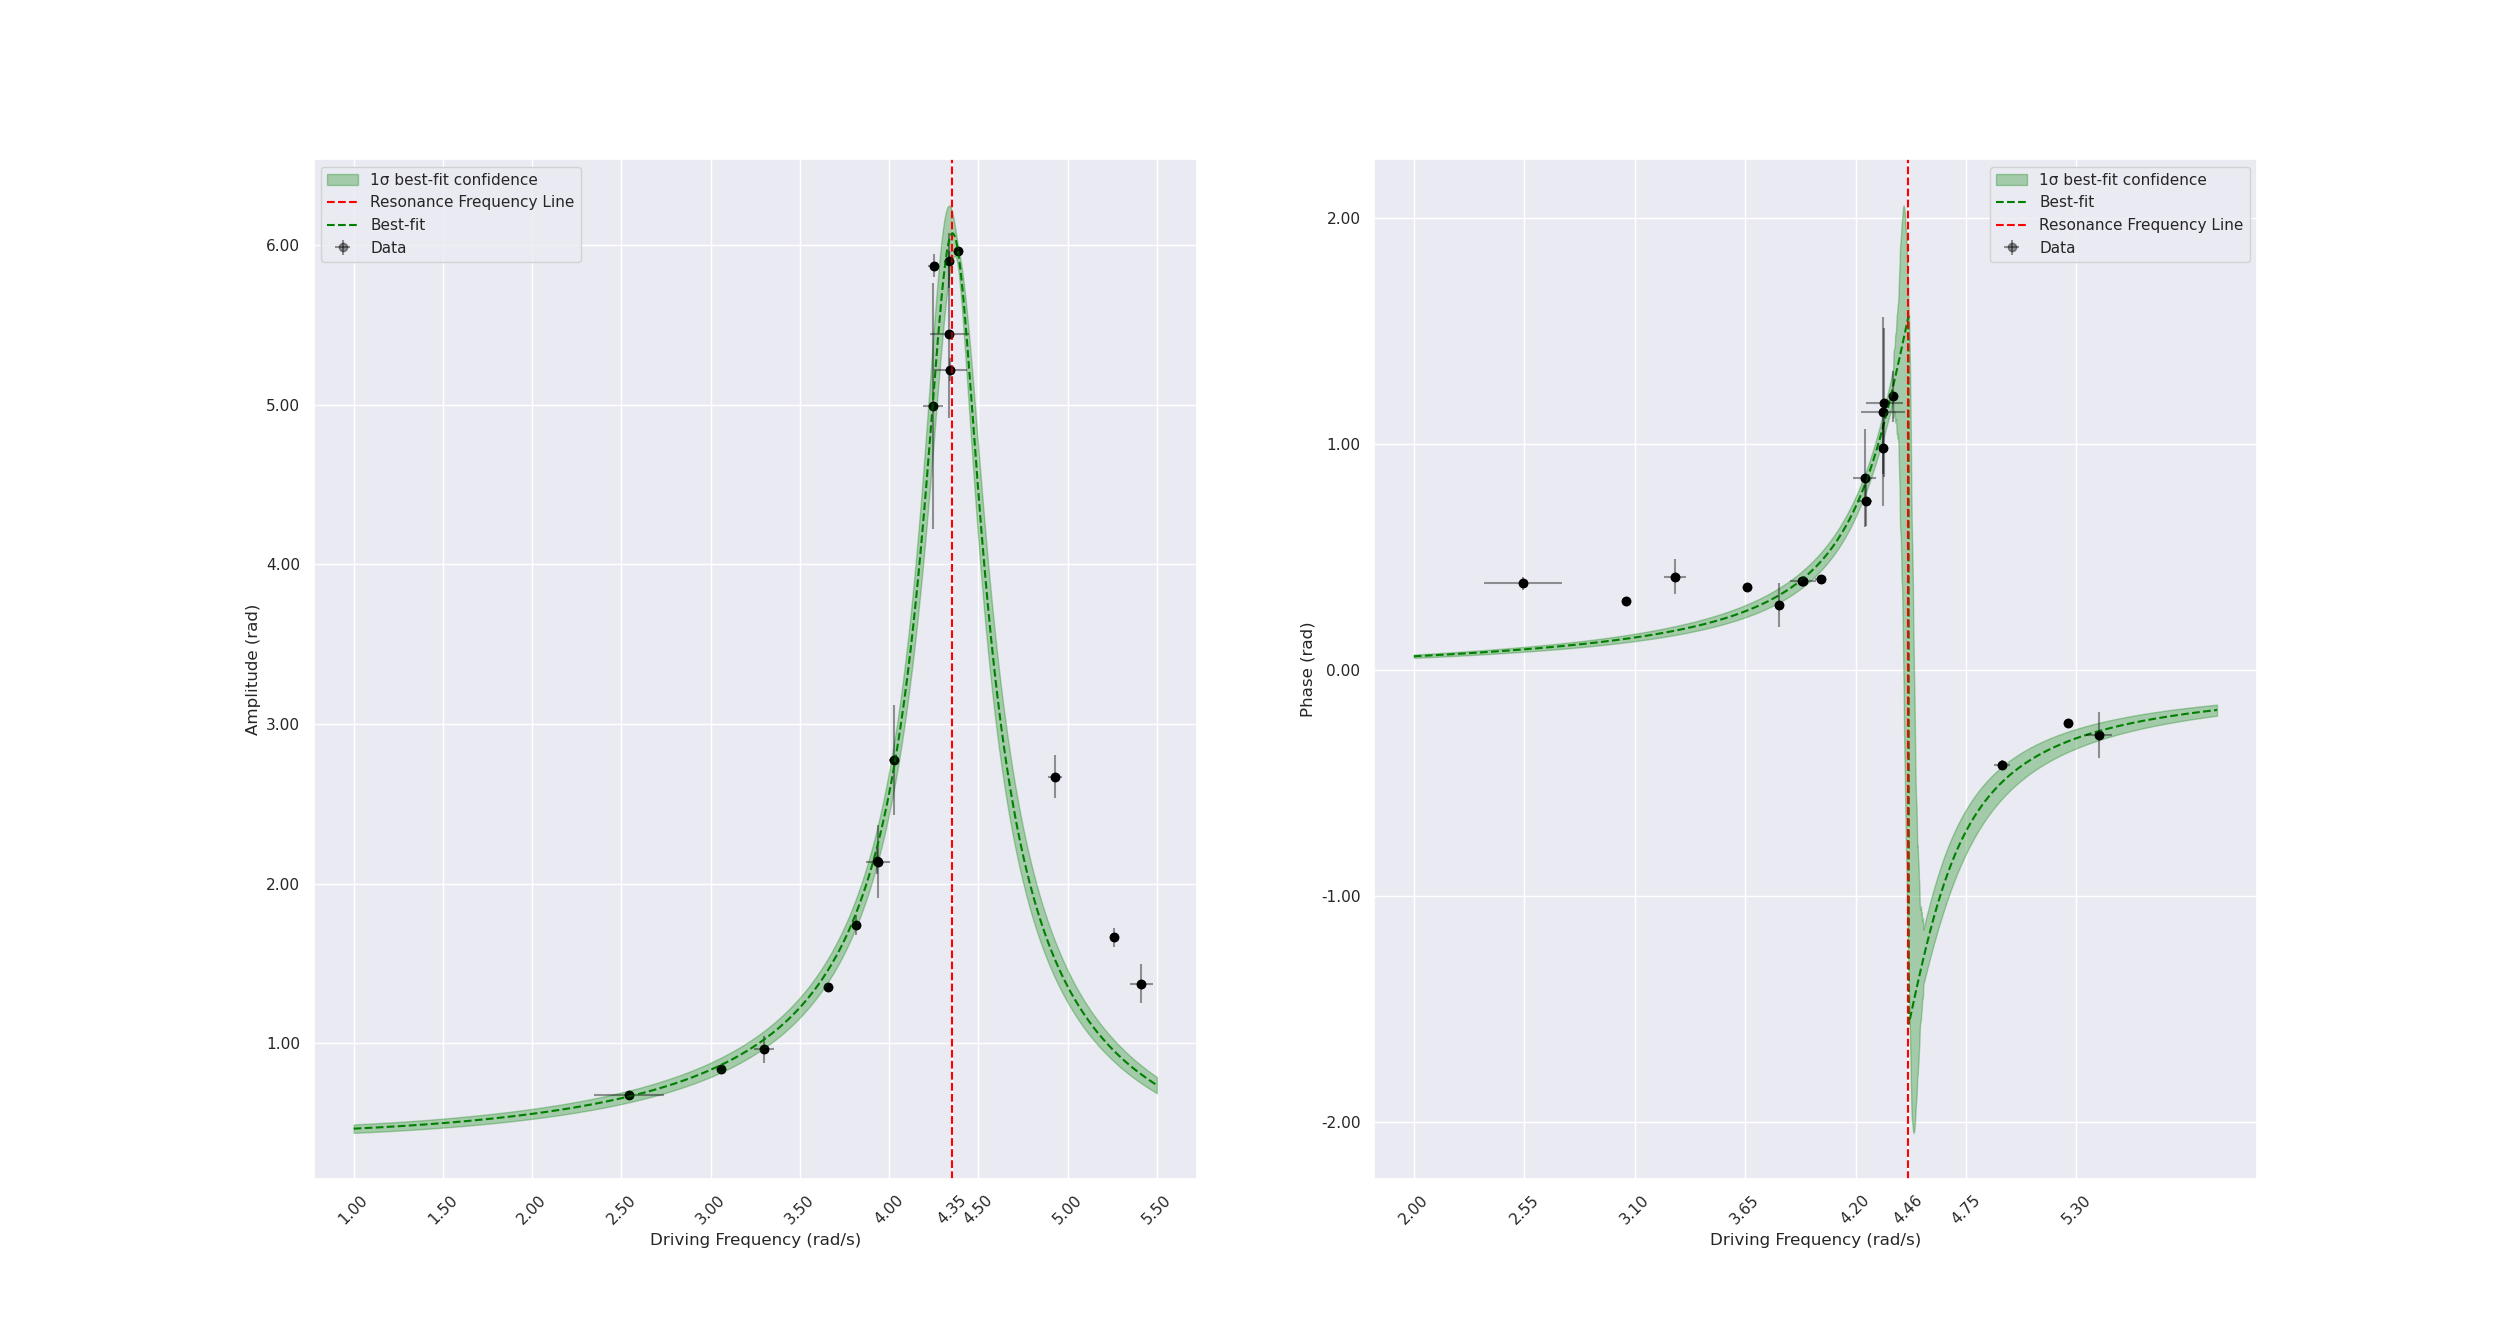
\includegraphics[width=1\textwidth]{oscillations/images/resonance}
  \caption{Amplitude and phase difference of the oscillations plotted against driving frequency.}
  \label{fig:resonance}
\end{figure}

The graph of the amplitude and phase difference of the oscillations against driving frequencies with best-fit curves and correspoding uncertanties are depicted in Fig.\ref{fig:resonance}. Tabular data with respective errors are depicted in Table \ref{tab:data}.

Resonance frequency from the amplitude-frequency graph is estimated to be $\omega_{amplitude} = 4.35 \pm 0.09 (rad/s)$. Resonance frequency from the phase-frequency graph is estimated to be $\omega_{phase} = 4.46 \pm 0.02 (rad/s)$. Combined resonance frequency is

\begin{equation*}
\omega_{r} = \frac{\omega_{amplitude} + \omega_{phase}}{2} \pm \sqrt{\sigma(\omega_{amplitude}) + \sigma(\omega_{phase})} = 4.41 \pm 0.09 (rad/s)
\end{equation*}

Damping factor is again evaluated from Eq.~\ref{eq:freq_deps}.

\begin{equation*}
        \gamma = \sqrt{ \frac{\omega^2 - \omega_{res}^2}{2} } = \sqrt{ \frac{4.79^2 - 4.41^2}{2} } = 1.32 \pm 0.8 (rad/s)
\end{equation*}       

This damping factor matches the damping factor previously calculated in a different way.

Error analysis for the resonance frequencies and the damping factor is located in Appendix \ref{appendix:errors}.
